\chapter{Forward Solutions}\label{ch:fwd}

\section{Overview}

As described previously, the forward problem predicts the potentials observed along some measurement surface (commonly the body surface) given a set of known electrical sources and the geometry through which those source fields conduct. In this chapter, we will provide an overview of the forward problem as it is implemented in the Fwd/Inv toolkit, which generally calculates torso surface potentials given a set of known cardiac source parameters. Of course, these toolkit networks can be manipulated to incorporate other source models (\eg{} brain potentials or transmural cardiac potentials) or solution representations (\eg{} scalp or epicardial potentials) as needed.

The forward problem can be broken down into two fundamental concepts: 1) how to represent the source and 2) how that source maps to desired observation locations (\eg{} torso surface). One can conceptualize these two concepts in the classic sense by considering the function $\mathbf{y}(t) = \mathbf{A}\mathbf{x}(t)$,  where $\mathbf{y}(t)$ (Eq.~(\ref{eq:TransMat})) represents a set of unknowns on the torso surface (observation locations) and $\mathbf{x}(t)$ is the cardiac source or source formulation. The function $A$, therefore, represents how source potentials are to be mapped to the observation field and is dependent on the choice of source model, the solution approach (\ie{} FEM/BEM), and relevant torso specific requirements such as conductivities and geometry.

The two most common source formulation models used in cardiac forward problems are cardiac potentials and activation times. The use of cardiac potentials is arguably a more intuitive formulation in that it is typically potentials that are recorded from cardiac-specific electrodes.  Activation times must be {\em derived} from recorded signals and are, therefore, one step removed from the original recordings.  In terms of abbreviated physiology, cardiac potentials relate the interaction of cardiac cells to changes in the extracellular potential fields of the myocardium. These extracellular cardiac potentials are then projected to the torso surface. The activation-time-based source formulation, on the other hand, deals with the fact that when inactive and active tissues exist in close proximity, a source much like a dipole or layer of dipoles can be generated that is representative of the propagating activation wavefront, which then projects to the torso surface. Both of these source models contain several assumptions, but each provides a generally accurate model that can be computationally reasonable.

With the source formulation considered, one must now determine the pattern with which that source projects to the torso surface. As mentioned, this relationship is dependent on the choice of source model, the solution approach, and the various properties of the torso. In both source models presented, the function $A$ can be represented by an $N \times M$ matrix where $N$ is the number of points on the cardiac surface and $M$ is the number of points on the torso surface.  This matrix representation is called the lead field, or transfer, matrix. Calculating this matrix can be computationally intensive, and there are several ways to approach it. The two examples provided in the Fwd/Inv toolkit find the lead field, or transfer matrix, based on finite element (FEM) and boundary element methods (BEM). The theory and mathematics behind these two methods are presented in Ch.~\ref{sec:math}.

We provide in this toolkit three methods to calculate the forward problem. Potential based models using both FEM and BEM are demonstrated, as well as an activation-time based model using FEM.
The activation based model in its current state, however, is incomplete.
The network is provided, though it is still undergoing a series of improvements.
% || EDIT ME: || once the network is again availabe.
The BEM activation-time forward problem is not yet supported in SCIRun, though a working version is available through ECGSim, the interactive simulation software developed by Peacs in the Netherlands. ECGSim assumes an equivalent dipole layer as the approximated source in the activation based forward problem and is compatible with SCIRun outputs.\footnote{To obtain this free software, visit http://www.ecgsim.org/. Any references to ECGSIM herein are referring to version 1.3 beta}

The general network structure of all forward problems in the Fwd/Inv toolkit can be broken down into 6 component phases: Phase 1: Data Inputs, Phase 2: Parameter Manipulation \& Transfer Matrix Computation, Phase 3: Solution Calculation, Phase 4: Data Mapping, Phase 5: Visualization, and Phase 6: Data Output (though most networks provided omit the final phase).
Descriptions using these phases will be utilized throughout each network description below.

\section{Module Descriptions for Boundary Element Solutions}

The boundary element solution utilizes many common modules within the SCIRun framework
to read in files, visualize data, and manipulate geometry. Descriptions of these modules
can be found in the SCIRun documentation, whereas the modules that are relatively unique to the boundary element solution are outlined below.

Following the format proposed above, the BEM Solutions network in the Fwd/Inv toolkit is broken up into only the first five phases.
\begin{itemize}
\item {\bf Phase 1: Data Inputs} \\
Cardiac (source) and torso (measurement/solution space) geometries as well as cardiac source potentials are read into the network.  Additional fields are provided in the actual Fwd/Inv toolkit network that are unique to validating the specific model as well.  This is because both heart and torso potentials are known for this example, both torso and heart data are available to be read in and used to simulate and validate the problem.  As such, alternative geometries representing recorded torso potential sites with their associated recorded potentials are also included.
\item {\bf Phase 2: Parameter Manipulation \& Transfer Matrix Computation} \\
Modules assign source and measurement surfaces within the formulation and the conductivities between these respective surfaces as well as (if necessary) provide a means for defining/re-assigning surface normals.
\item {\bf Phase 3: Solution Calculation} \\
With Data Inputs representing vector $x$ of our linear system and the Transfer Matrix $A$ being computed, the next step is to solve for $b$ using the equation $Ax = b$.
\item {\bf Phase 4: Data Mapping} \\
The solution to our problem involves a full time series of data inputs that were read in as part of Phase 1. Extracting a single time step from the solution and mapping it to the respective torso geometry is necessary for subsequent visualization.
\item {\bf Phase 5: Visualization} \\
SCIRun offers an interactive visualization environment that is more thoroughly covered in the Basic SCIRun Tutorial documentation. Briefly, visualizations in the Fwd/Inv toolkit allow the user to display the source and solution geometries with data values mapped and colored onto each respective surface.  The view window allows the user to then interactively manipulate the view orientation in order to generate the optimal visualization for the purposes of explaining the data.
\end{itemize}

Unique to the BEM implementation in SCIRun is the {\tt BuildBEMatrix} module (Figure \ref{fig:BuildBEModule}).
This module accepts only surface inputs into a dynamic port structure, meaning that as additional inputs are added, additional input ports will appear ({\em notice the 3rd input port in Figure \ref{fig:BuildBEModule} even though only 2 inputs are provided}).
A minimum of two surfaces must be used, though support for multiple surfaces is available.
Generally, the initial input (input port 1) will accept the inner surface representing the source.
The last output is reserved for the final outer measurement field (usually the torso) with all additional fields representing regions internal to the measurement field surface but external to the source surface (\eg{} lungs, bone, and other internal torso structures).

\begin{figure}[H]
\begin{center}
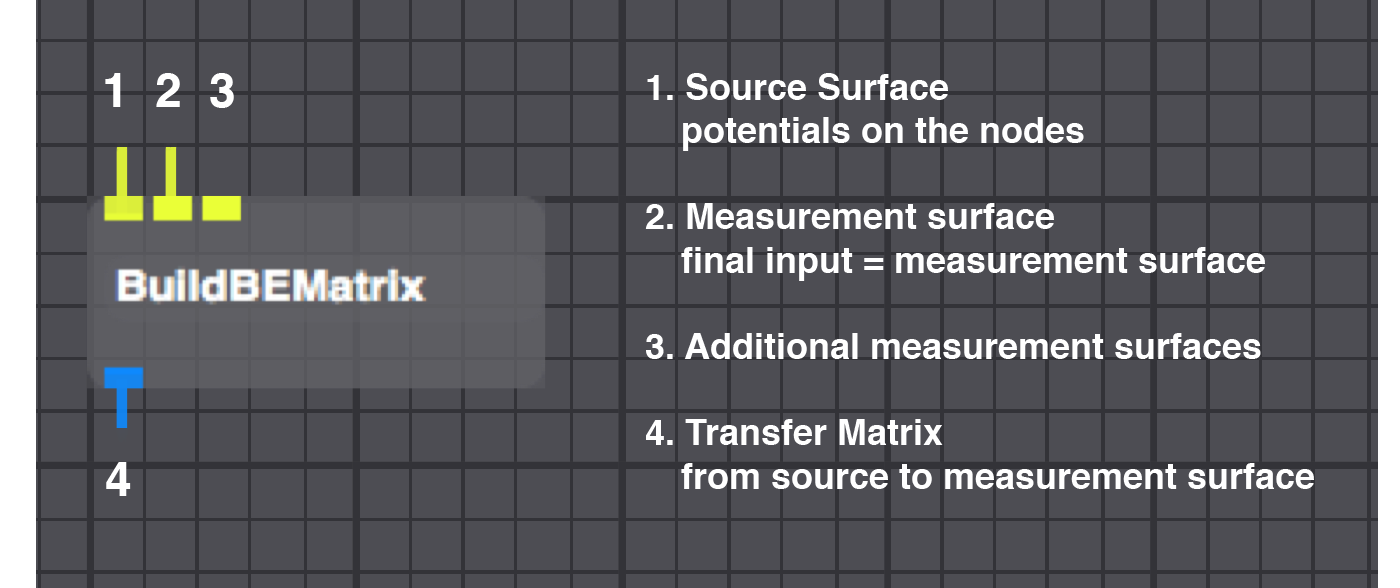
\includegraphics[width=.8\textwidth]{ECGToolkitGuide_figures/BEMmod.png}
\caption{{\bf BuildBEMatrix Module.} The {\tt BuildBEMatrix} module computes the transfer matrix between
the source surface and the outermost measurement surface.}
\label{fig:BuildBEModule}
\end{center}
\end{figure}

\newpage

\begin{figure}[t]
\begin{center}
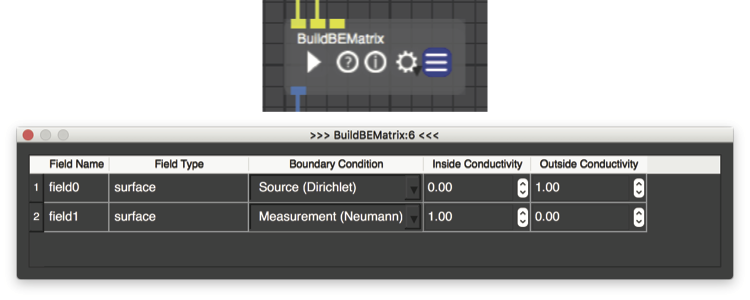
\includegraphics[width=\textwidth]{ECGToolkitGuide_figures/BuildBEUI_combined.png}
\caption{{\bf BuildBEMatrix Module Interface.} The {\tt BuildBEMatrix} UI allows the user to define boundary
conditions and conductivities within the mesh. }
\label{fig:BEM_UI}
\end{center}
\end{figure}
% .8 textwidth is used to match the height of all of the module description images.  AddKnownsToLinearSystem is a longer module, and therefore a longer image.  The size reductions in BuildBEMatrix and BuildFEMatrix are used to match the AddKnowns image.

\begin{wrapfigure}{r}{0.49\textwidth}
\begin{center}
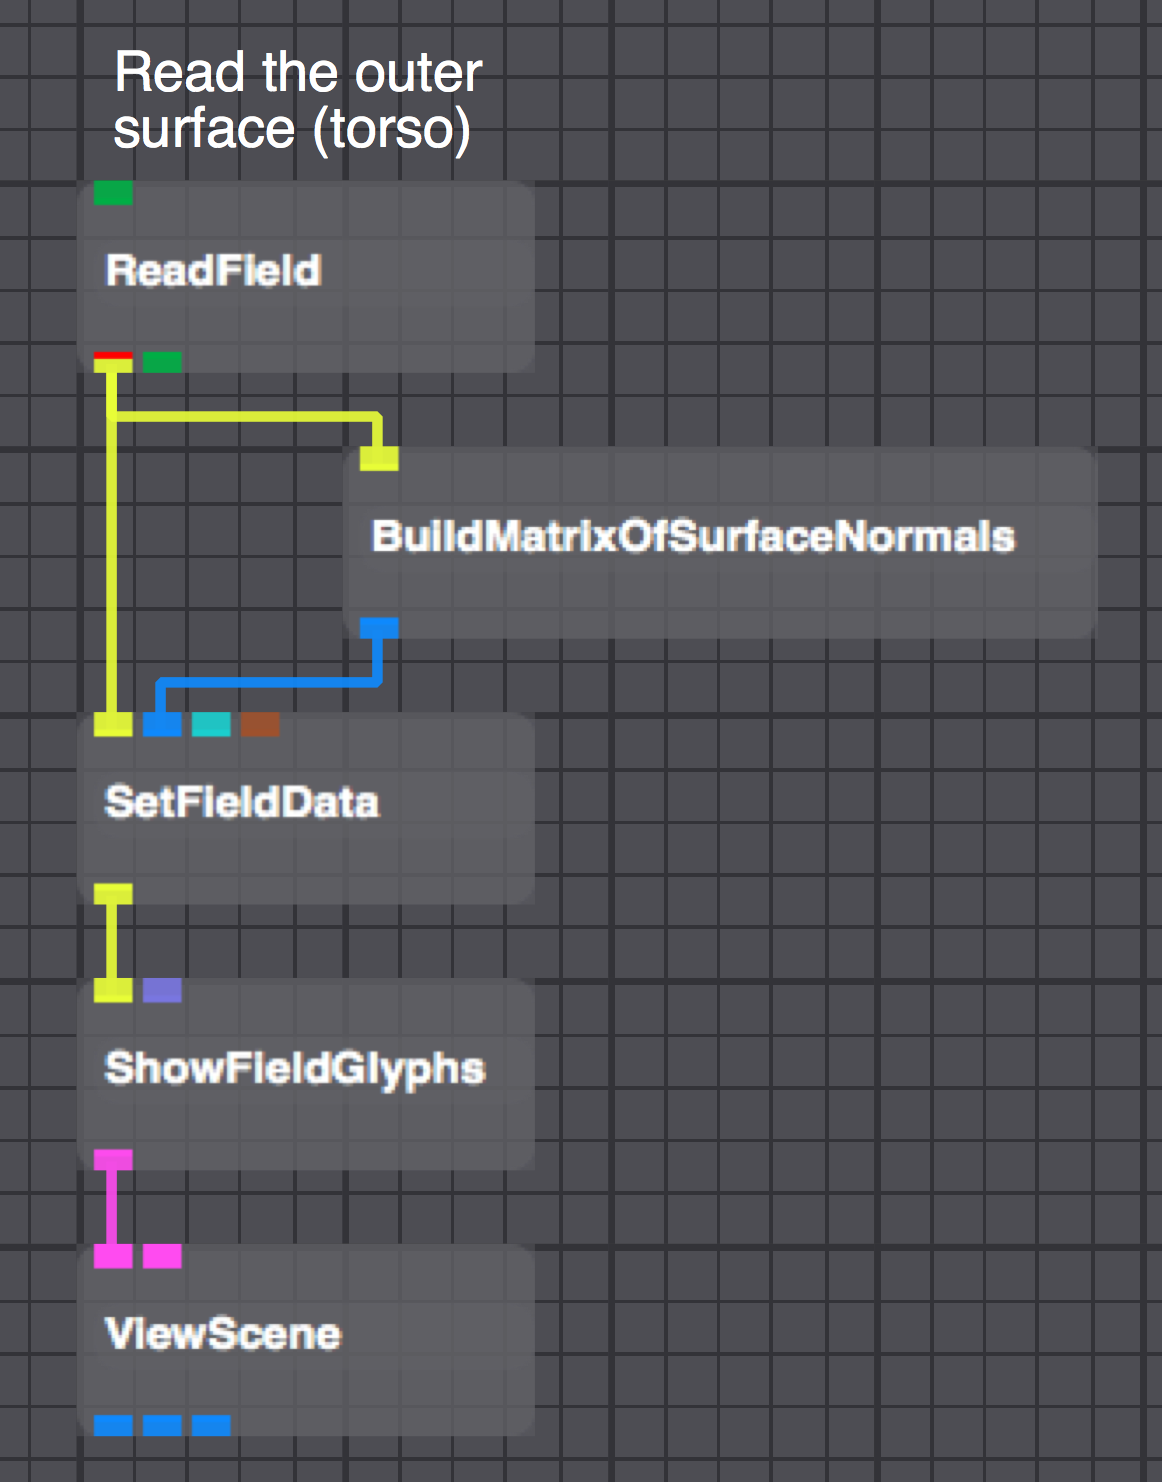
\includegraphics[width=.45\textwidth]{ECGToolkitGuide_figures/CheckSurfaceNormals.png}
\caption{{\bf Checking Surface Normals.} Checking surface normals requires the creation of a surface normal matrix that is then mapped back onto the original surface geometry. Showing field vectors as arrows allows the user to determine surface normal directions.}
\label{fig:CheckNormals}
\end{center}
\vspace{-.25in}
\end{wrapfigure}

Hovering over the {\tt BuildBEMatrix} module produces a display of icons used to investigate and manipulate the module.
The user interface (UI) icon is the right-most icon comprising three horizontal lines.
Accessing the UI, as shown in Figure \ref{fig:BEM_UI}, allows the user to define surface specific parameters such as boundary conditions and conductivity values within the surfaces.
Users should be careful to match conductivity values with respect to each surface.
For example, in Figure \ref{fig:BEM_UI}, the outside source conductivity matches the inside conductivity of the torso surface.

Contrary to traditional BEM approaches, the {\tt BuildBEMatrix} assumes that, for any closed surface, the surface normals will be pointing {\em inward} -- not outward. The surface
normal for each element is defined using the right hand rule (counterclockwise) of the node order in each element.
The module {\tt FlipSurfaceNormals} can be used to flip all the element normals on the surface.
It is important to check
the normals of model surfaces because incorrect normals will produce erroneous answers.
Figure \ref{fig:CheckNormals} shows a simple way to check surface normals in SCIRun using the module chain, or snippet.

\newpage

\section{Module Descriptions for Finite Element Solutions}

The two most important modules for the forward finite element solution are the {\tt BuildFEMatrix}
and the {\tt AddKnownsToLinearSystem} modules. {\tt BuildFEMatrix} allows the user to compute a stiffness matrix while {\tt AddKnownsToLinearSystem} provides a means for adding boundary conditions to the system.
The {\tt BuildFEMatrix} module receives a finite element mesh and an optional look up table (LUT) matrix of conductivity values.
To simplify the assignment of conductivity values, the user can simply define conductivity values directly onto each element in which case, the LUT input port should be left unconnected.
If the the lookup table method is preferred, the user must make sure that integer values are assigned to the mesh that correspond to the index numbers within the lookup table that contain the proper conductivities for each respective region.
The resulting output of the {\tt BuildFEMatrix} module is a stiffness matrix for the mesh that was generated using the Galerkin method with linear basis functions.

\begin{figure}[t]
\begin{center}
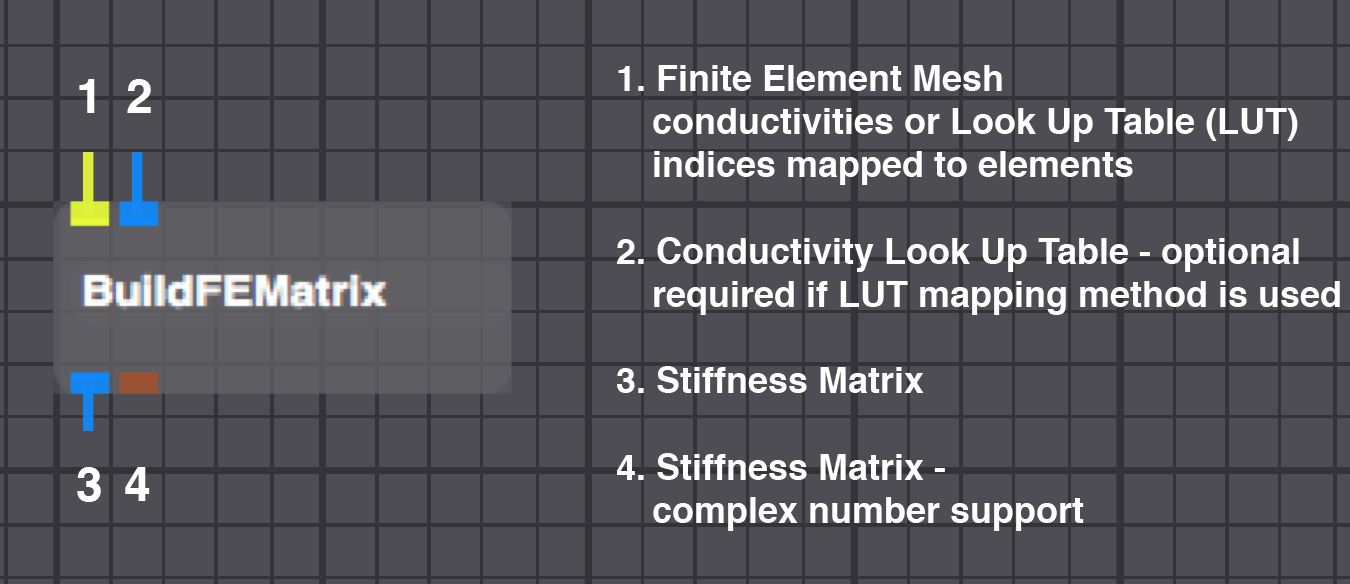
\includegraphics[width=.8\textwidth]{ECGToolkitGuide_figures/BuildFEMatrix.png}
\caption{{\bf BuildFEMatrix Module.} The {\tt BuildFEMatrix} module that computes the stiffness matrix for a FEM solution.}
\label{fig:FEM}
\end{center}
\end{figure}

\begin{figure}[b]
\begin{center}
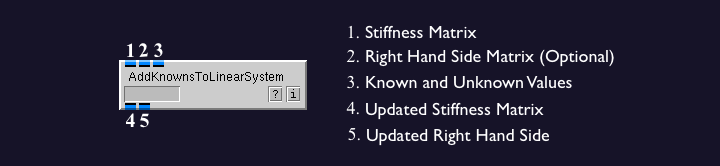
\includegraphics[width=\textwidth]{ECGToolkitGuide_figures/AddKnowns.png}
\caption{{\bf AddKnownsToLinearSystem Module.} The {\tt AddKnownsToLinearSystem} module recalibrates  the stiffness matrix and RHS vector for a FE solution given known values in $\mathbf{x}(t)$ and (optionally) $\mathbf{y}(t)$.}
\label{fig:AddKnowns}
\end{center}
\vspace{-.25 in}
\end{figure}

{\tt AddKnownsToLinearSystem} makes it possible to add known values as boundary conditions
to the linear system $\mathbf{y}(t) = \mathbf{A}\mathbf{x}(t)$, where some values of
$\mathbf{x(t)}$ are already known.
The module receives the stiffness matrix $\mathbf{A}$ along with an $\mathbf{x(t)}$ matrix with known values imposed at the specific indices where data is known and $NaN$ values occupying the remaining vector entries.
A right-hand-side (RHS) matrix may also be provided if any of the solution values are also known, but it is not required.
If an RHS field is not included then it is assumed that the vector contains all zeros. % | Is this true...it isn't NaNs?
Using the provided inputs, the module adjusts the linear system according to the known values.
This means that $\mathbf{A}$ and the RHS vector $\mathbf{y}(t)$ are altered in such a way that the product of the new stiffness matrix and RHS $\mathbf{(A2)^{-1}} \mathbf{b2}$ (referring to Figure \ref{fig:AddKnowns}) will produce an $\mathbf{x(t)}$ that contains the defined values at the specified locations.

%\newpage
\section{Example Networks for Boundary Element Solutions}

The following network shows the most basic implementation of the boundary element method (Figure \ref{fig:BEMnet})
along with a visualization of the results (Figure \ref{fig:BEMsol}). To follow our previous standard:
\begin{itemize}
\item {\bf Phase 1: Data Inputs} \\
A torso mesh and epicardial surface mesh with associated data matrix of epicardial potentials at each node is read into the network.
\item {\bf Phase 2: Parameter Manipulation \& Transfer Matrix Computation} \\
The conductivities of the torso and heart are set, along with the differentiation between source and measurement surfaces as shown in Figure \ref{fig:BEM_UI}, and a transfer matrix is computed.
\item {\bf Phase 3: Solution Calculation} \\
The transfer matrix is applied to the vector representing the potentials along the epicardium in the form of the equation $\mathbf{Ax = b}$.
\item {\bf Phase 4: Data Mapping} \\
The solution is then mapped to the torso surface.
\item {\bf Phase 5: Visualization} \\
Finally, the results are visualized and displayed using SCIRun's {\tt ShowField} module.
\end{itemize}



\newpage

\begin{figure}[H]
\begin{center}
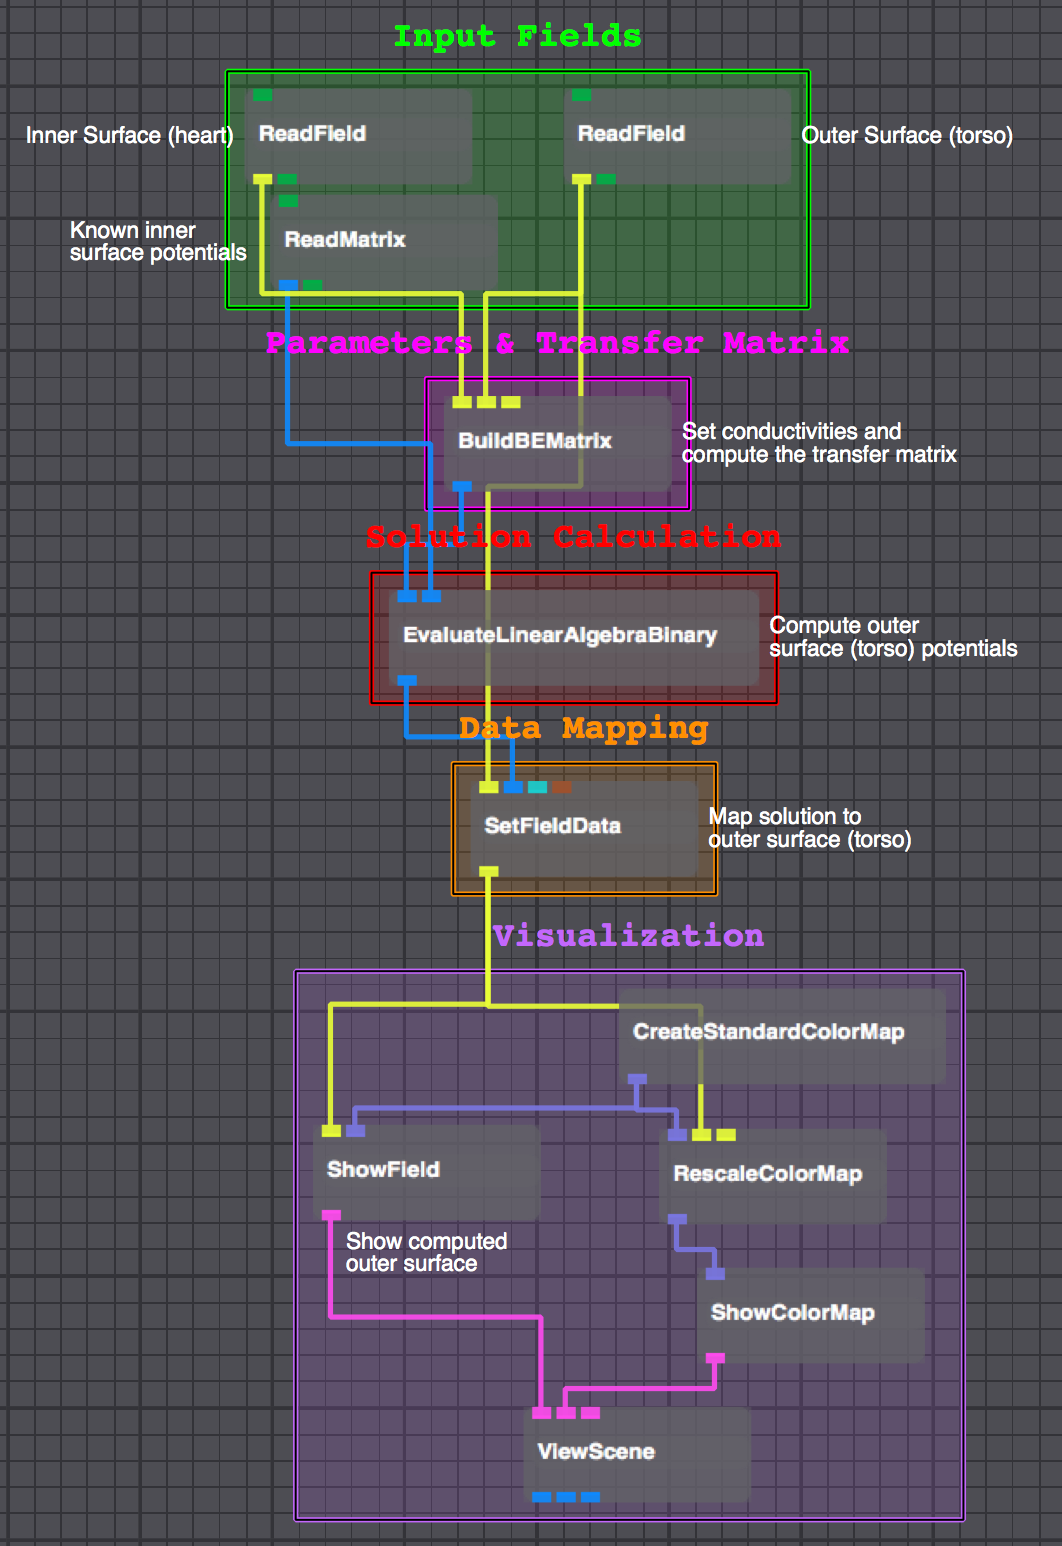
\includegraphics[width=.9\textwidth]{ECGToolkitGuide_figures/BEMnetwork.png}
\caption{{\bf BEM Network Example.} A simple implementation of the boundary element method in SCIRun.}
\label{fig:BEMnet}
\end{center}
\vspace{-.25in}
\end{figure}

\textit{A similar SCIRun network for this example can be found in the Fwd/Inv toolkit at:\\{\tt [ToolkitPath]/Networks/potential-based-bem/torso-tank-bem.srn5}}

\begin{figure}[H]
\begin{center}
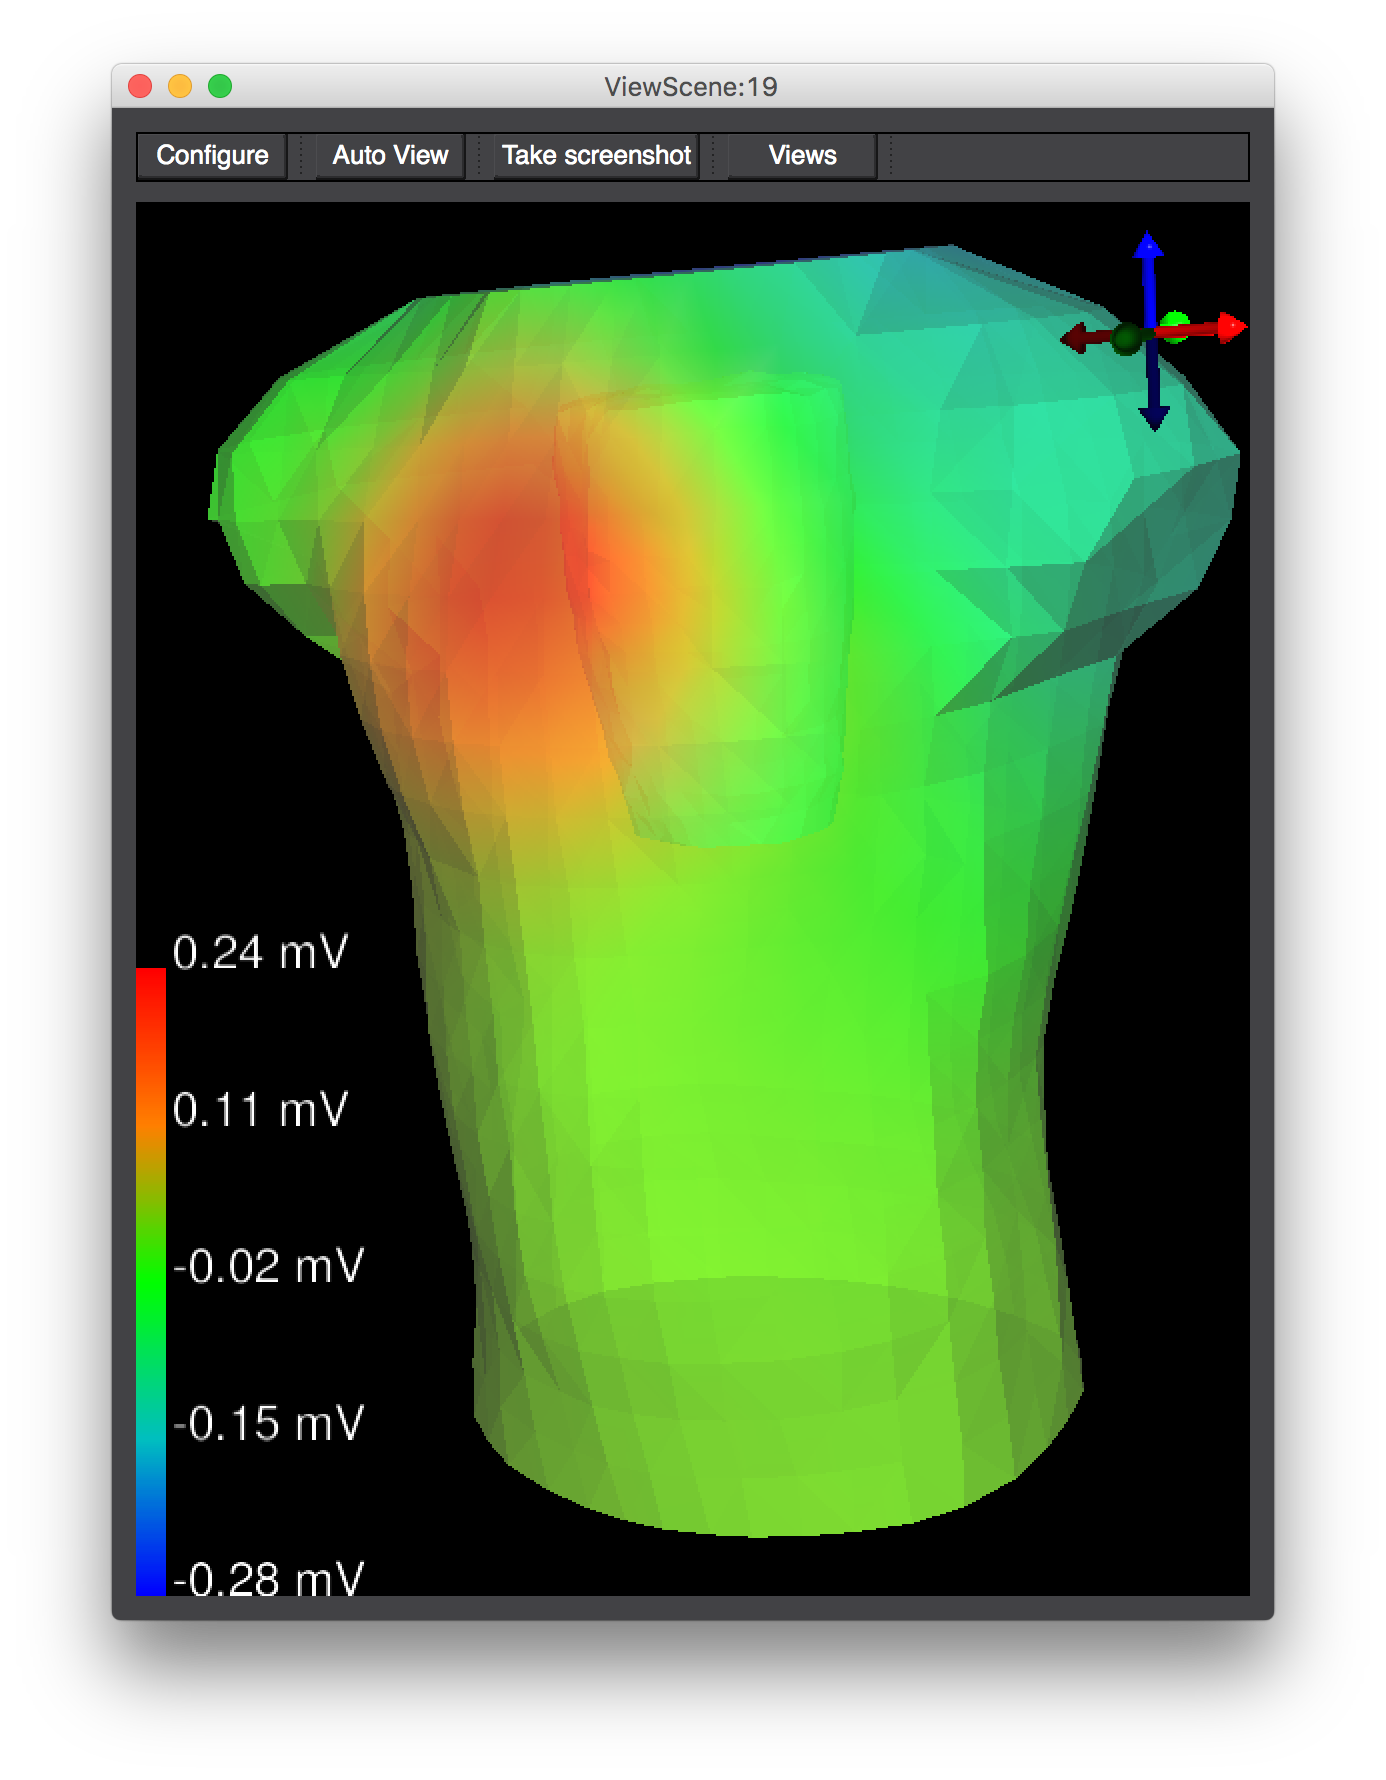
\includegraphics[width=.9\textwidth]{ECGToolkitGuide_figures/BEMSolution.png}
\caption{{\bf BEM Solution Example.} Potentials from the internal surface (representing the heart potentials) were computed to the torso surface. An additional {\tt ShowField} module was used in the above network (Figure \ref{fig:BEMnet}) to display the cardiac region.}
\label{fig:BEMsol}
\end{center}
\vspace{-.25in}
\end{figure}

\newpage

\section{Example Networks for Finite Element Solutions}

There are two examples in the Fwd/Inv toolkit for calculating the potential-based forward problem using finite element method. The first example is a direct calculation of the projection of the cardiac potentials into the torso mesh, satisfying Laplace's equation, and from thence to the torso surface.
The second example involves the generation of the lead field matrix, or transfer matrix, that is then used  to perform the forward calculation that very much resembles the $\mathbf{y}(t) = \mathbf{A}\mathbf{x}(t)$ formulation seen in the BEM method above.

\subsection{Potential Based Forward FEM Simulation: Laplacian Solve}

The following example network shows a basic implementation of the finite element method used to solve Laplace's equation in order to, in essence, project cardiac surface potentials throughout the torso and onto the torso surface (Figure~\ref{fig:PotBasedFEM_Lap}).
Though this problem is not formulated in the classic sense of the forward problem, it is useful because it does not require calculating a lead field matrix, which is often limited to a low resolution domain due to the extensive time required to compute the lead field matrix.
In each example it is assumed that the input meshes need no additional manipulation.
The actual networks housed in the Fwd/Inv toolkit use torso segmentation files as meshes that need moderate regional geometric parsing in order to obtain the desired mesh.
In this network time-series data is provided, but a solution for the time-series cannot be computed in a single step as was done in the BEM solution.
Using the FEM approach with time-series input requires that the potential values at each desired time instant be extracted using the {\tt GetFieldSlice} module.
These data are subsequently mapped to the heart before an FEM solution is generated (Figure \ref{fig:PotBasedFEM_Lap}).

As mentioned previously, the Laplacian Solve method implemented in this network uses Laplace's equation to solve for torso potentials. That is, all the potentials in the torso satisfy the expression:
\begin{equation*}
\nabla \sigma \nabla \phi = 0
\end{equation*}
\noindent where $\phi$ are the potentials within the torso mesh and $\sigma$ are the conductivity values. Using SCIRun, one is able to use the cardiac surface potentials as known values and solve the rest of the torso potentials to satisfy Laplace's equation as a linear system.
The network is organized, again, in the following manner.

%The example network\\
%{\tt potential-based-fem/forward\_problem\_with\_lead\_field\_matrix.srn} is a network that computes the forward problem in a more traditionally understood method (Figure~\ref{fig:pot_for_fem_w_mat}), in that it is a simple matrix multiplication to calculate the torso potentials. This network simply uses a pre-computed lead field matrix and multiplies it by the cardiac potentials to yield the surface torso potentials. Different time points may be selected in the {\tt GetColumnOrRowFromMatrix} module.


\begin{itemize}
\item {\bf Phase 1: Data Inputs} \\
A labeled torso mesh and epicardial surface mesh with associated time-series data matrix of epicardial potentials over several time instances is read into the network.
\item {\bf Phase 2: Parameter Manipulation \& Transfer Matrix Computation} \\
Potential data are mapped into the torso mesh (right). Notice the need for geometric manipulation (left) in order to remove the heart from the torso. With the mesh prepped a LUT approach is used to generate map conductivities into the FEM matrix.
\item {\bf Phase 3: Solution Calculation} \\
Known values are added to the linear system before an iterative solver is used to compute the solution.
\item {\bf Phase 4: Data Mapping} \\
The solution is then mapped to the torso and its surface is extracted.
\item {\bf Phase 5: Visualization} \\
The results are smoothed using the {\tt FairMesh} module and visualized.
\end{itemize}

\begin{figure}[H]
\vspace{-.25in}
\begin{center}
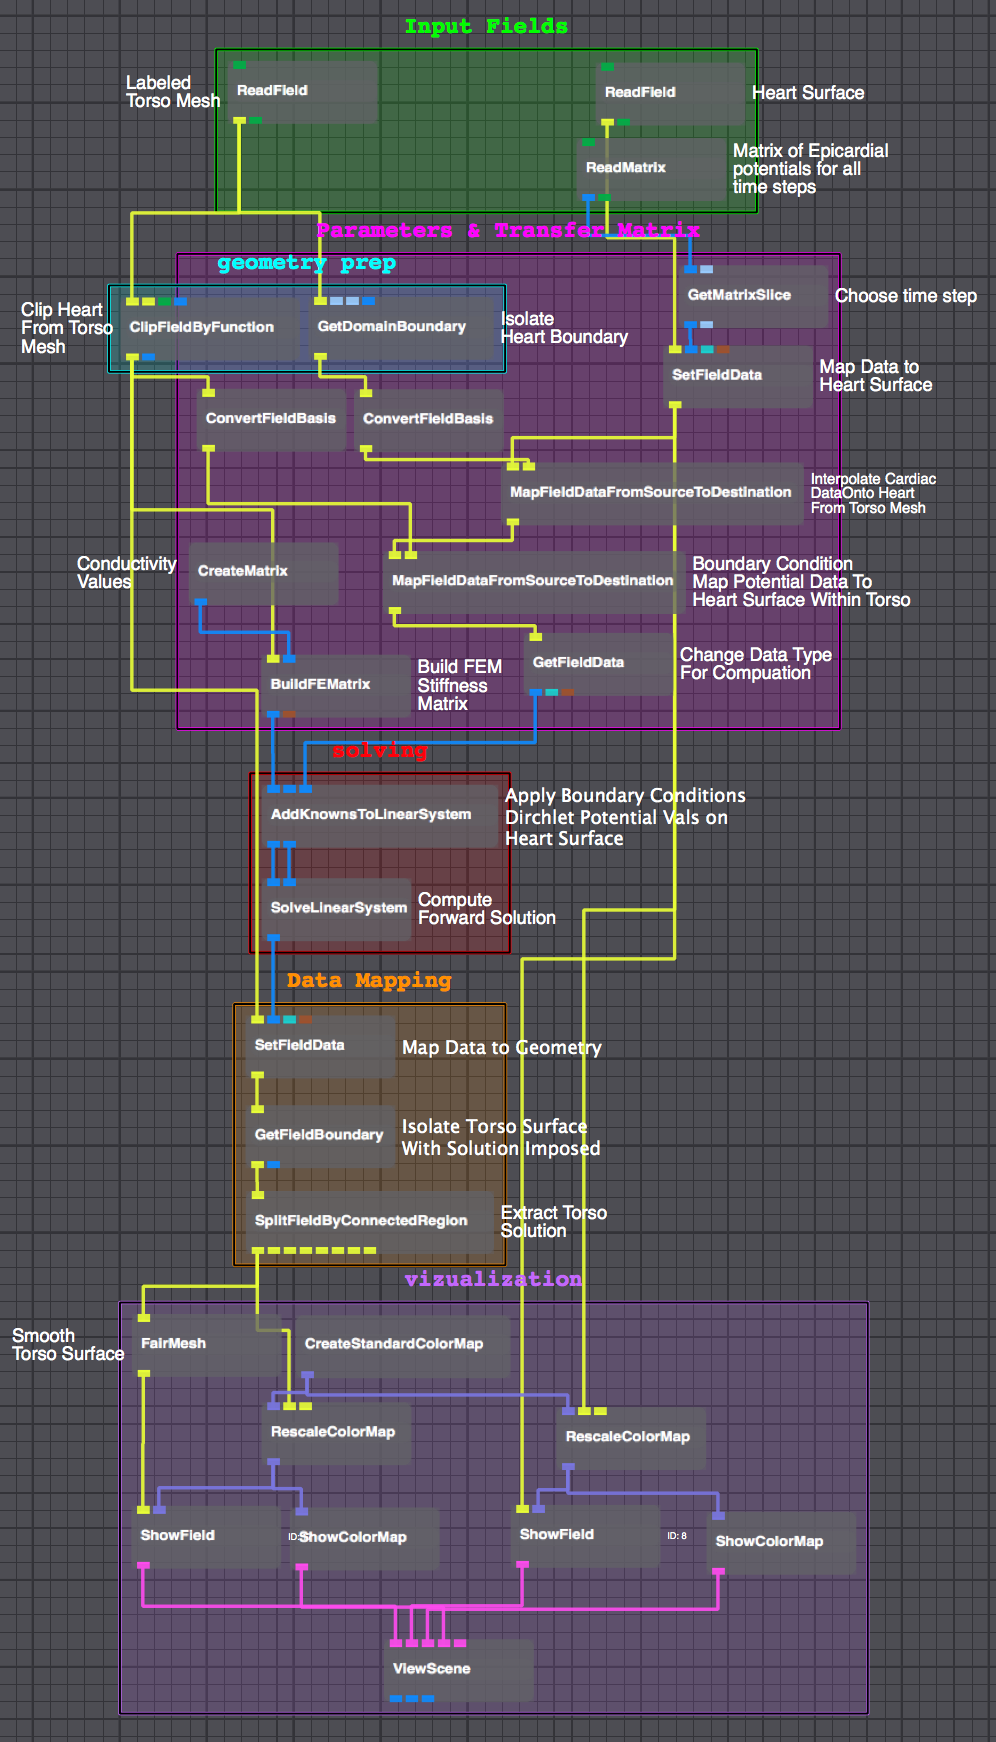
\includegraphics[width=.7\textwidth]{ECGToolkitGuide_figures/PotBasedFEM_Lap.png}
\caption{{\bf FEM Network Example.} A simple implementation of the finite element method in SCIRun.}
\label{fig:PotBasedFEM_Lap}
\end{center}
\vspace{-.25in}
\end{figure}

\begin{figure}[H]
\vspace{-.25in}
\begin{center}
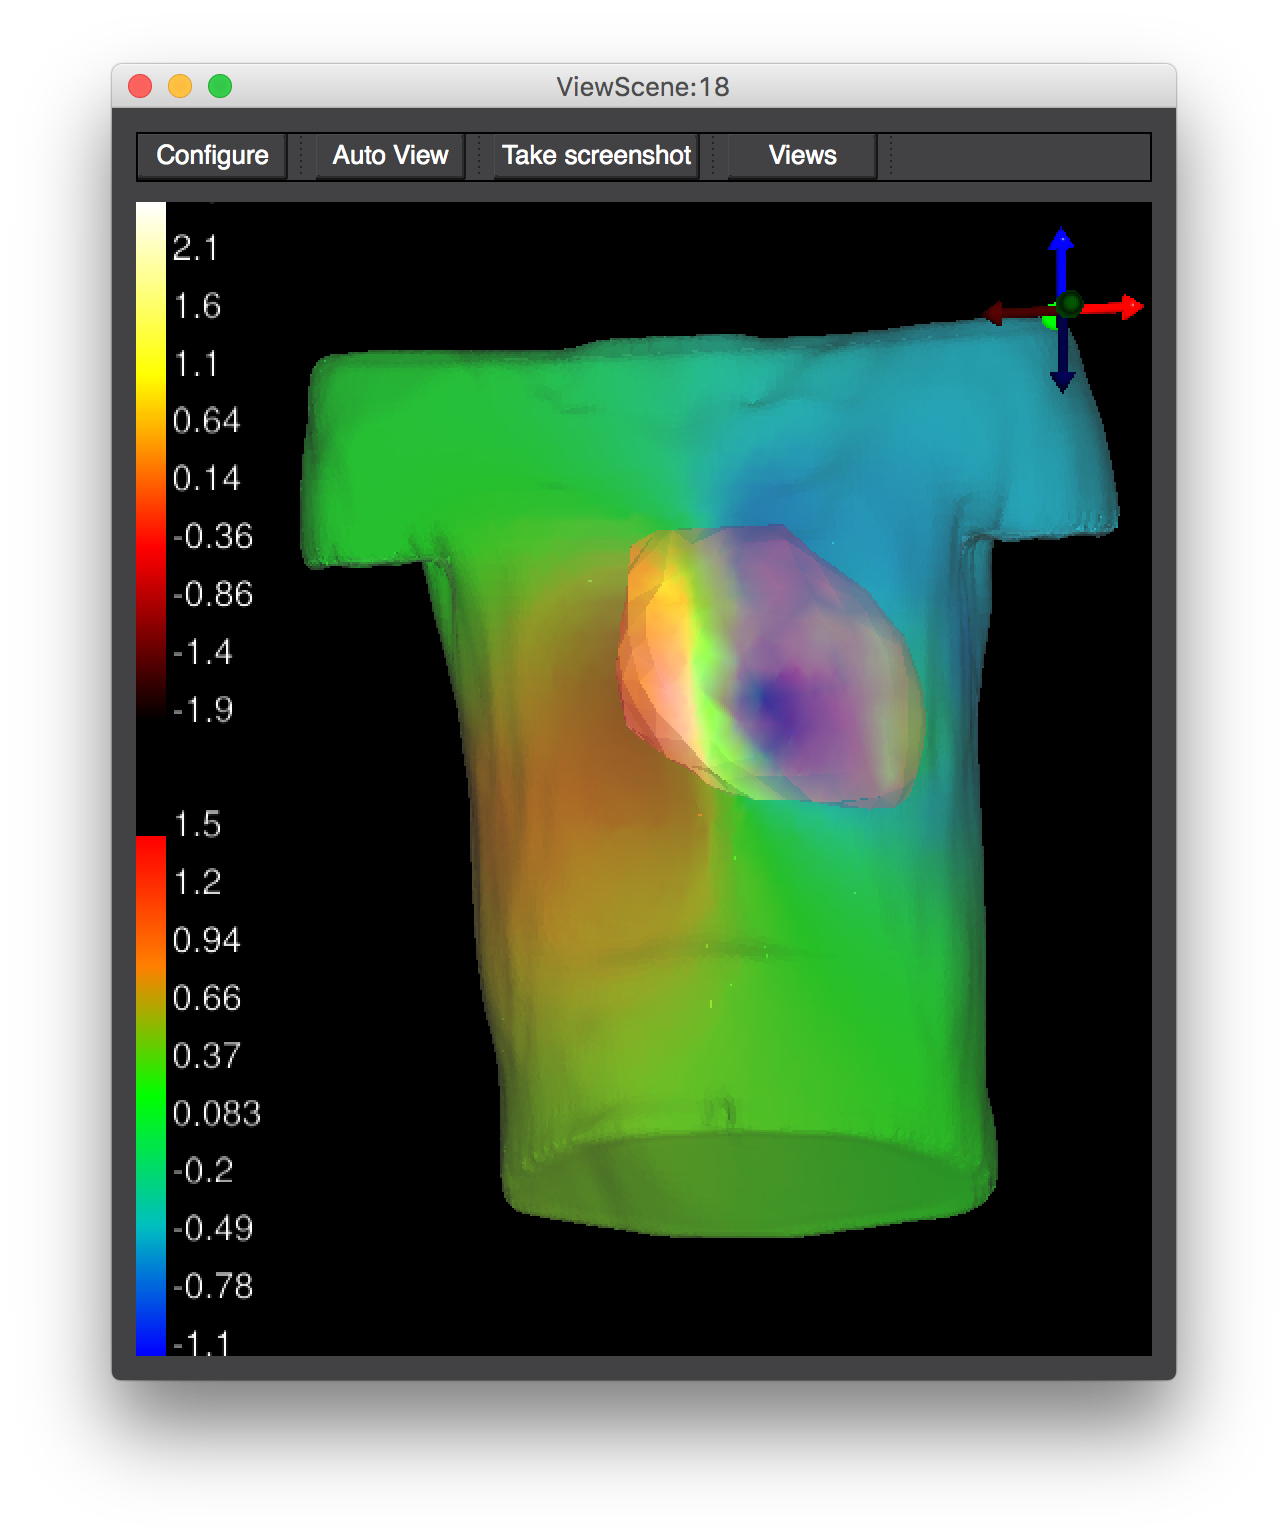
\includegraphics[width=\textwidth]{ECGToolkitGuide_figures/PotBasedFEM_LapSol.png}
\caption{{\bf FEM Laplace Solution Example.} Laplace's equation was solved within the torso to project potentials from the heart throughout the torso domain. The torso surface was subsequently extracted and visualized.  Different colormaps have been assigned to the heart (source) and the torso (solution) surfaces.}
\label{fig:PotBasedFEM_LapSol}
\end{center}
\vspace{-.25in}
\end{figure}

\textit{A similar SCIRun network for this example can be found in the Fwd/Inv toolkit at:\\{\tt [ToolkitPath]/Networks/potential-based-fem/forward\_problem.srn5}}

\subsection{Potential Based Forward FEM Simulation: Lead Field Calculation}

The following example utilizes two networks in order to produce 1) a lead field matrix with which to solve
2) a traditional $\mathbf{y}(t) = \mathbf{A}\mathbf{x}(t)$ forward solution.
Figure \ref{fig:FEMLead} shows a basic implementation of the finite element method used to calculate a lead field matrix and Figure \ref{fig:FEM_LeadNet} shows how that lead field matrix can be applied to generate a forward solution.
These networks also show the complete networks available in the Fwd/Inv toolkit in all their complexity.
Input meshes are segmentations that include multiple label masks (including one for the heart volume with a closed epicardium), which require manipulation prior to use.
%%%%%%%%%%%%%%%%
%Source potential values along the epicardial surface are imposed into the network and the solution across the entire mesh volume is obtained, though only the torso surface potentials are displayed.
%To calculate the lead field matrix, an identity matrix is also used for input vectors.

It is worth noting that the initial network, shown in Figure \ref{fig:FEMLead}, is remarkably similar to the Laplacian Solve network used in the previous section (Figure \ref{fig:PotBasedFEM_Lap}).
Apart from the additional geometric manipulation steps, that isolate the heart and torso regions, the major difference between these two networks is the definition of source potentials.
The Laplacian solution (Figure \ref{fig:PotBasedFEM_Lap}) applies a potential field to the nodes along the surface of the heart.
That is, it applies a complete data set in which each node has a specified potential value that is representative of the potential measurements along the epicardium at a given time instance.
The motives for using the heart potentials as a source is to be able to interpolate the response of the torso to potentials measured on the cardiac surface.
The goal of the lead field matrix creation approach (Figure \ref{fig:FEMLead}) is different.
The lead field matrix aims to define the relationship between the source and the solution spaces in global terms -- not just as a response to potentials during a single step in time.
This global relationship is defined by identifying the influence that each source node has on the entire system -- similar to the generation of a transfer matrix in the BEM approach.
First, a single source node is ``activated" (given a value of 1) while the other nodes are ``inactive" (given a value of 0).
The Laplacian is computed via an FEM approach, producing a solution vector that defines the influence of the active node on the system.
The data makes up one column of the lead field matrix.
A second node is then activated while all others are left inactive, creating another column in the lead field matrix.
This process is repeated for every source node and the results are collected producing an $N$ x $M$ matrix, where $N$ is the number of nodes defining the source, and $M$ is the number of nodes in the complete solution space.

Because we are computing the lead field matrix separately from the actual forward computation, a 6th phase is added to the process in which we save out the data field.
A practical implementation of data collection when executing the lead field matrix generation network is the need to:
\begin{enumerate}
\itemsep-.25em
\item Set the three {\tt CollectMatrices} settings to ``Column", ``Append", and ``PostPend"
\item Clear any previous data in the {\tt CollectMatrices} module using the ``Clear Output" button in the module UI.
\item Set the {\tt GetMatrixSlice} module at 0 before pressing play.
\end{enumerate}

Once a lead field matrix is generated and saved, it can be used in a relatively simple network to generate a forward solution for any set of data points that are applied to the heart (Figure \ref{fig:FEM_LeadNet}).
Notice that in Phase 2 (Parameter Manipulation \& Transfer Matrix Computation) no transfer matrix is computed.
This is because the lead field acts as the transfer matrix, which is now one of the Input fields.
As one would expect, comparing the solution of the Lead Field Solution (Figure \ref{fig:FEM_LeadSol}) to those of the Laplacian Solution (Figure \ref{fig:PotBasedFEM_LapSol}) -- taken at the same time step -- yields very similar results with only slight discrepancies in the upper range of the matrix.


%Choosing between Laplacian or Lead Field solution approaches is a matter of  preference and convenience.
%On the one hand, Laplacian solutions are quick and relatively simple to execute; on the other hand, they are not the traditional approach to forward computation.  Computing the lead field matrix is useful when executing several forward calculations on the same geometry, but the production of the lead field matrix is time intensive and computation time should be taken into consideration when deciding which forward approach to use.

\newpage

\begin{figure}[H]
\vspace{-.25in}
\begin{center}
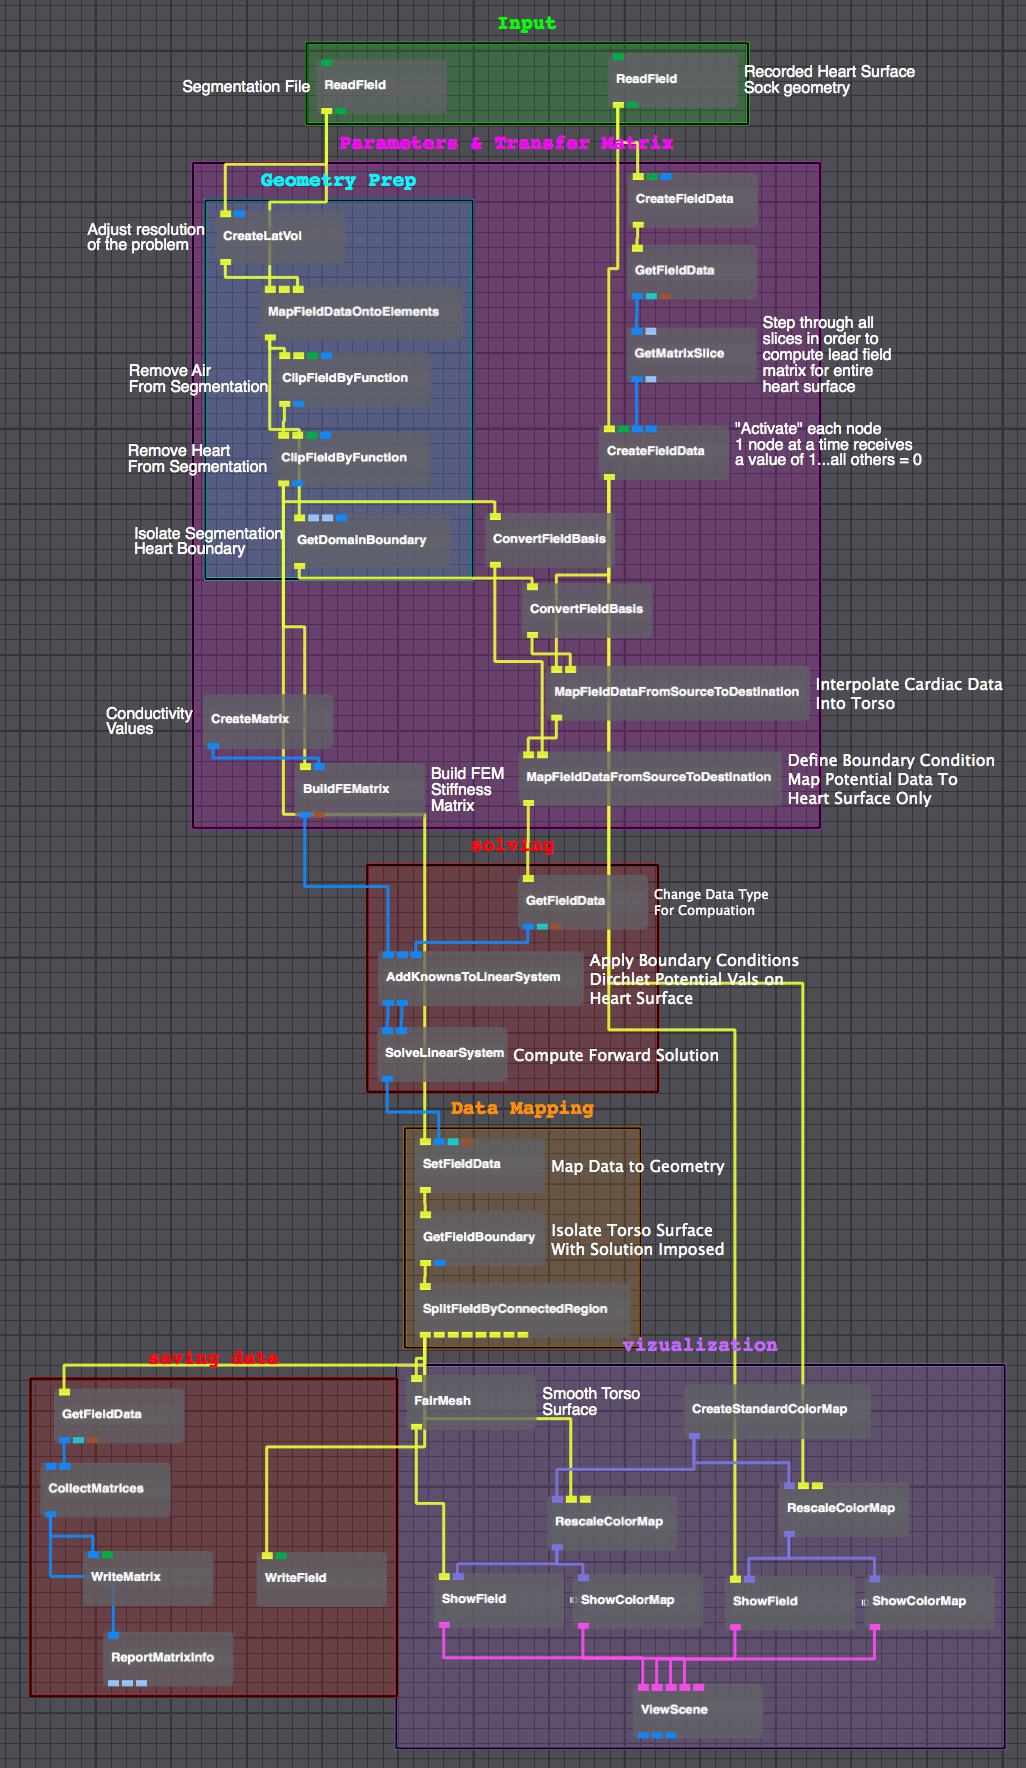
\includegraphics[width=.75\textwidth]{ECGToolkitGuide_figures/FEMLead.png}
\caption{{\bf FEM Lead Field Generation Example.} A network that demonstrates the creation of a lead field matrix in SCIRun.}
\label{fig:FEMLead}
\end{center}
\vspace{-.25in}
\end{figure}
\noindent
The lead field matrix provided was generated by the network \newline
{\tt [ToolkitPath]/Networks/potential-based-fem/make\_lead\_field\_matrix.srn5}.

\begin{figure}[H]
\begin{center}
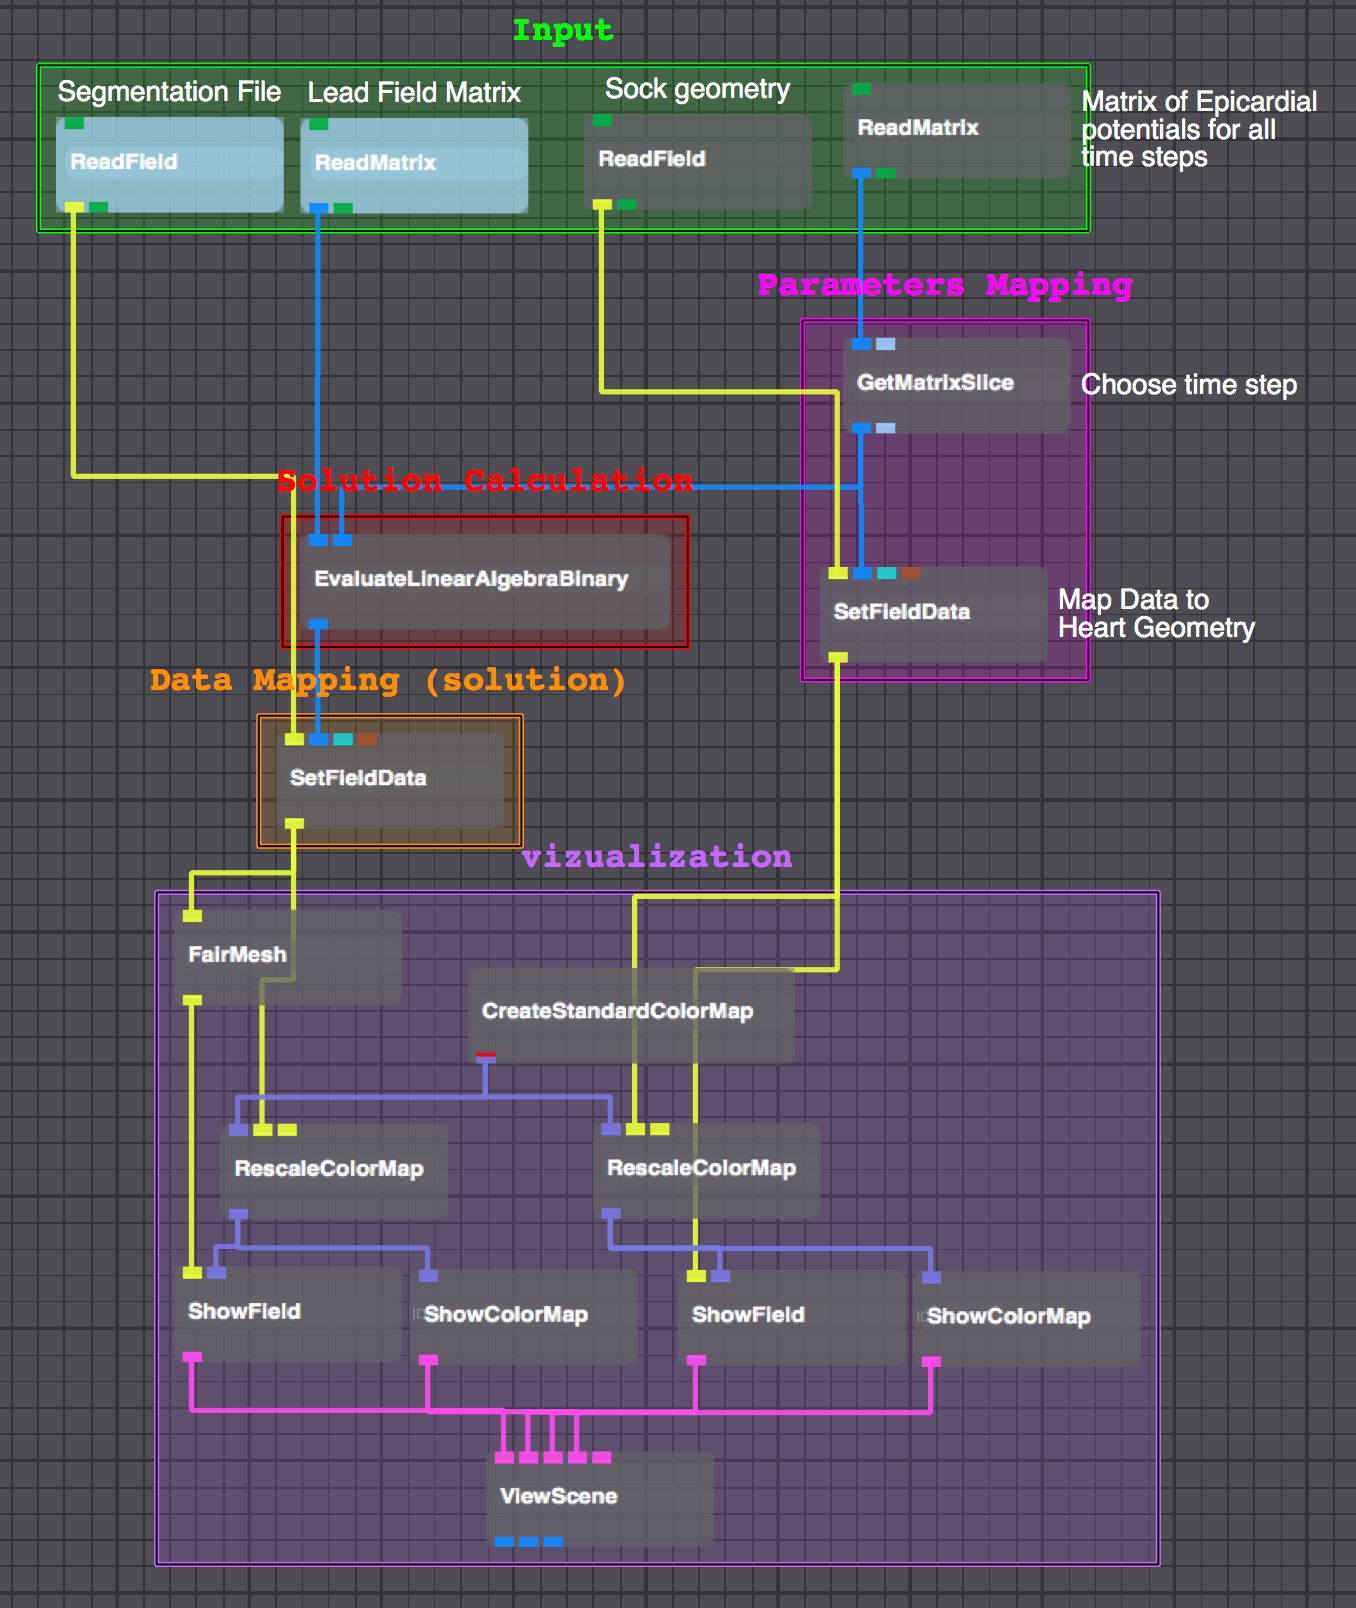
\includegraphics[width=\textwidth]{ECGToolkitGuide_figures/FEM_LeadNet.png}
\caption{{\bf FEM Lead Field Solution Example.} A network that demonstrates how to use a lead field matrix to solve the cardiac forward problem.}
\label{fig:FEM_LeadNet}
\end{center}
\end{figure}
\noindent
The FEM solution with lead field matrix provided was generated by the network \newline
{\tt [ToolkitPath]/Networks/potential-based-fem/... \\Forward\_problem\_with\_lead\_field\_matrix.srn5}.

\begin{figure}[H]
\begin{center}
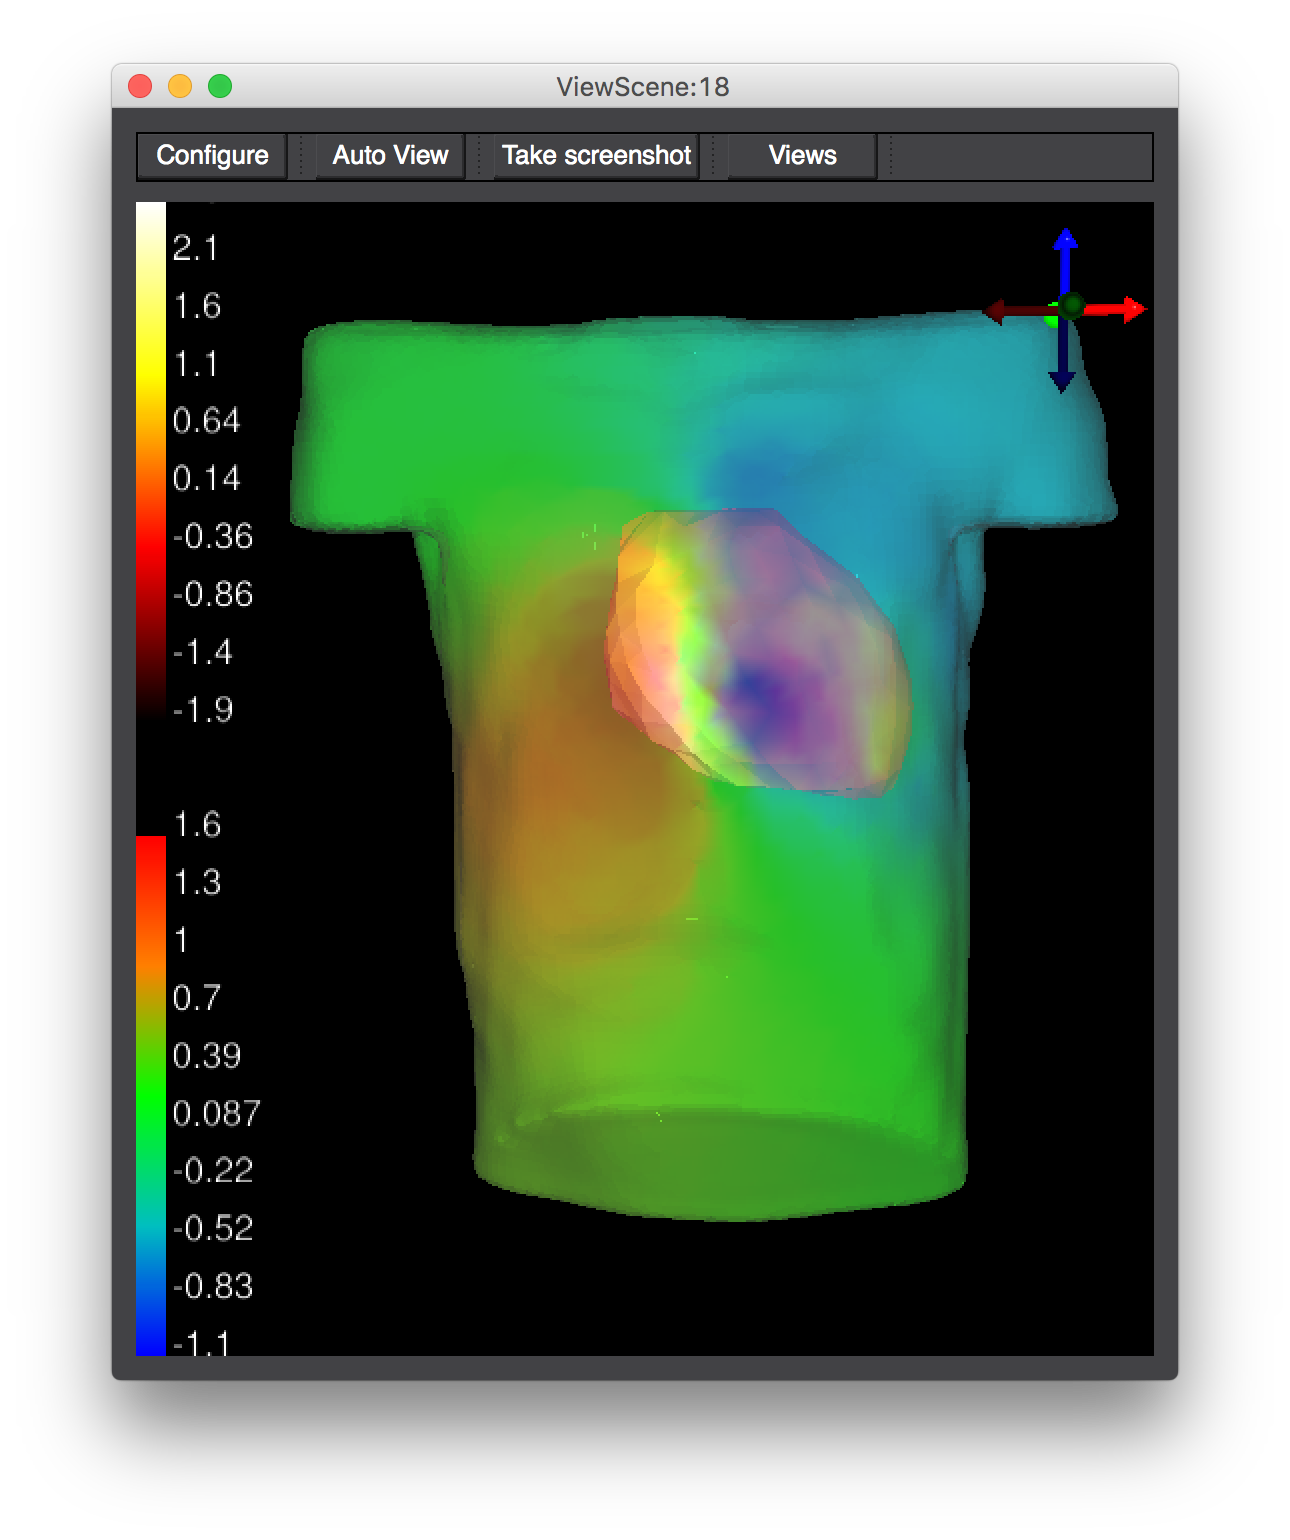
\includegraphics[width=\textwidth]{ECGToolkitGuide_figures/PotBasedFEM_LeadSol.png}
\caption{{\bf FEM Lead Field Solution Example.} The product of Figures \ref{fig:FEMLead} and \ref{fig:FEM_LeadNet} the lead field solution produces similar results to those produced by the Laplacian solution (Figure \ref{fig:PotBasedFEM_LapSol}) when considering the same time step.}
\label{fig:FEM_LeadSol}
\end{center}
\end{figure}

\subsection{Activation Based Forward FEM simulation}


\paragraph{}As stated above, the activation-based model is incomplete and under review.
If the reader has any practical experience and/or would like to assist in the
development and implementation of this network, please contact us using the
contact information provided in the introduction.
%
%The technique used by the activation-based model is quite different from
%the potential-based approach.
%Activation-based methods, instead of searching solely for the
%potentials, consider whether a region of the heart is ``active'' or ``inactive".
%In other words, it considers the profile of the source potentials at a tissue level.
%The activation profile is used to specify the strength, in time, of
%dipoles located on the surface.
%
%Since FEM is a volume-based method, the dipoles used to generate a wavefront
%are computed within the volume. This is done by assigning SCIRun approximates the volume potentials
%by first clipping it with the surface mesh of the inner and outer boundaries.
%With this, it obtains a volume mesh that roughly follows the surface. Then, the
%potentials of this volume mesh are set so that they approximate the dipoles
%on the heart surface. This representation is known as the equivalent dipole
%layer.
%
%There are three networks located in {\tt  src/nets/FwdInvToolbox/activation-based-fem}
%which provide an example of activation-based forward calculation
%using FEM. The three networks are similar in nature to the potential-based
%FEM forward problem networks explained in Sec.~\ref{sec:pot_for_fem}.
%The activation-based forward problem networks use data derived from ECGSIM.
%The surface mesh and source parameters are also obtained from the ECGSIM
%project.
%
%The primary inputs to this network are the surface mesh representing
%the heart, a torso surface mesh which is made a volume mesh
%(refined near the surface of the heart) in the network, and
%a matrix specifying the activation profile for each point in the heart
%surface mesh at each time to be simulated. This matrix is then of size
%$N \times M$ where $N$ is the number of surface points and $M$ is the
%number of time-steps represented. A very good example of the input
%expected can be obtained from the ECGSIM software by choosing {\em
%Save $\rightarrow$ Source parameters} from the {\em File} menu.
%
%Though the {\tt activation-based-fem.srn} networks seem quite complicated,
%they perform some simple tasks. The loaded torso surface is made into a
%volume and refined in nearer to the heart. Then, two cardiac surfaces are
%made from the first, one slightly inside the heart, and one slightly outside.
%The corresponding points on the two surfaces are set to either active or inactive.
%If the point is inactive, then it is set as an unknown and will be solved for later. If
%the point is active, the two surfaces are set to opposing values to approximate a
%dipole layer. The remaining torso potentials are solved using a linear-systems
%solver similar to Sec.~\ref{sec:pot_for_fem}.
%
%The network {\tt activation-based-fem\_lead\_field.srn} produces similar results
%as the previous network, but it utilizes a pre-computed lead field matrix. This
%network allows for the activation times to be directly related to the torso surface
%and the computation is relatively quick. This method is also more like the
%traditionally formulated forward problem with a simple matrix multiply.
%
%The lead field matrix is calculated using the {\tt make\_lead\_field.srn} network.
%Similar to the potential-based approach (Sec.~\ref{sec:pot_for_fem}), the solution
%vectors for each point on the cardiac surface are calculated and collected as the
%lead field matrix. This is essentially a pre-computation of the contribution of each
%point. This calculation is very useful if the geometry is going to be used many times.
%
%
%To calculate the lead field matrix with {\tt make\_lead\_field.srn}:
%\begin{enumerate}
%\item{Make sure the {\tt CollectMatrices} module has not been executed.}
%\item{Set step delay in the {\tt GetColumnOrRowFromMatrix} module is set to a sufficient interval so that all the modules can fully execute before the next iteration.}
%\item{Set the current column to 0 and press ``play'' in the {\tt GetColumnOrRowFromMatrix}.}
%\item{After the network finishes iterating, enable the {\tt WriteMatrix} module (by right clicking on the module), choose the place and name of the matrix you would like, and press save.  }
%\end{enumerate}
%
%\begin{figure}[H]
%\begin{center}
%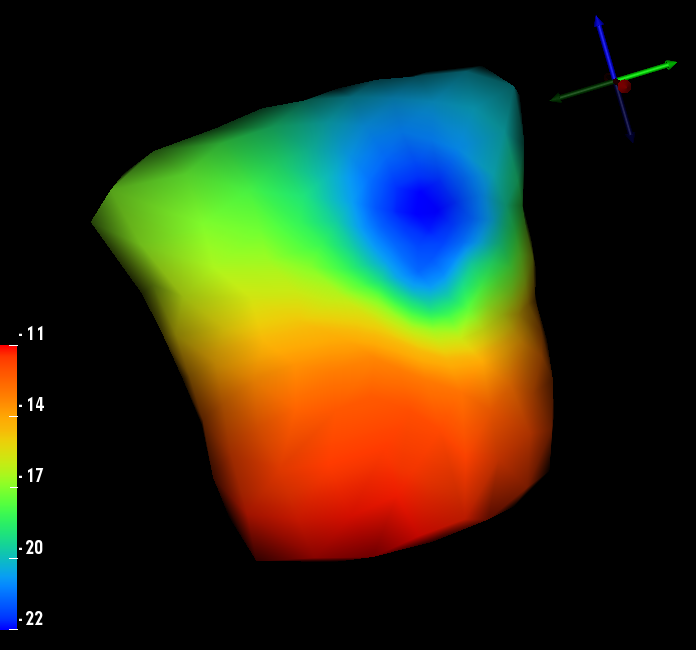
\includegraphics[width=\textwidth]{ECGToolkitGuide_figures/act_for_fem_results.png}
%\caption{Solution of the activation based forward problem using FEM.}
%\label{fig:act_fem_for_sol}
%\end{center}
%\end{figure}
